%!TEX root = PaulAllen_Y362220X_MST125_TMA_02.tex
\documentclass{tufte-handout}


\usepackage{style}
\usepackage{amssymb}


\newenvironment{amatrix}[1]{%
  \left(\begin{array}{@{}*{#1}{c}|c@{}}
}{%
  \end{array}\right)
}

\newenvironment{longdiv}[1]{%
  \(\begin{array}{r@{}*{#1}{c} r r}
}{%
  \end{array}\)
}

\begin{document}
\bibliography{biblio.bib} 
\tma{03}

%%%%%%Question 1

\begin{question}

\qpart

If if the following statments are true:

\begin{center}
\textit{If it is Robin's birthday, then Robin eats cake.}
\textit{Robin is eating cake.}
\end{center}

Let \( P \) be the statement "It is Robin's birthday" and \( Q \) be the statement "Robin eats cake".
The first statement can be written as \( P \implies Q \) and the second statement can be written as \( Q \).

The statment;
\begin{center}
\textit{It is Robin's birthday.}
\end{center}

\( P \) does not imply \( Q \).
Robin could be eating cake for any number of reasons. This is an example of the formal fallacy
affirming the consequences.

\vspace{3cm}

\qpart

\[ \text{For all positive integers } n, \text{ We have } 5^{n}\leq(6+1)^{6} \]

This can be proved false with;

\begin{align*}
\stext{Using \(n=9\)}\\
5^9 &= 1953125\\[8pt]
(9+1)^{6} &= 10^{6} = 1000000\\[8pt]
\stext{Thus }
1953125 &\leq 1000000 \text{ is false.}\\[8pt]
\end{align*}

\end{question}

%%%%%%%%%%%Question 2

\begin{question}

\qpart

    \[ y = \frac{4x-1}{3x-4} \]

\begin{align*}
\stext{Given \( x\neq\frac{4}{3} \) and \( y\neq\frac{4}{3} \)}
\stext{When \( x = \frac{4y-1}{3y-4}  \)}
y &= \frac{4x - 1}{3x - 4}\\[25pt]
&= \frac{4\left(\frac{4y-1}{3y-4}\right) - 1}{3\left(\frac{4y-1}{3y-4}\right) - 4}\\[25pt]
\stext{Distributing the \( 4 \) and \( 3 \)}
&= \frac{\frac{16y - 4}{3y - 4} - 1}{\frac{12y - 3}{3y - 4} - 4}\\[25pt]
\stext{Using the common denominator of \( 3y - 4 \)}
&= \frac{\frac{16y - 4 - (3y - 4)}{3y - 4}}{\frac{12y - 3 - 4(3y - 4)}{3y - 4}}\\[25pt]
\stext{Simplifying the numerator and denominator}
&= \frac{\frac{16y - 4 - 3y + 4}{3y - 4}}{\frac{12y - 3 - 12y + 16}{3y - 4}}\\[25pt]
&= \frac{\frac{13y}{3y - 4}}{\frac{13}{3y - 4}}\\[25pt]
\stext{Cancelling the common factor of \( 3y - 4 \)}
&= \frac{13y}{13}\\[8pt]
&= y
\end{align*}

\begin{align*}
\stext{Assume \( x = \frac{4y-1}{3y-4} \)}
\stext{Then \( y = \frac{4x-1}{3x-4} \)}
x &= \frac{4y - 1}{3y - 4}\\[25pt]
&= \frac{4\left(\frac{4x-1}{3x-4}\right) - 1}{3\left(\frac{4x-1}{3x-4}\right) - 4}\\[25pt]
\stext{Distributing the \( 4 \) and \( 3 \)}
&= \frac{\frac{16x - 4}{3x - 4} - 1}{\frac{12x - 3}{3x - 4} - 4}\\[25pt]
\stext{Using the common denominator of \( 3x - 4 \)}
&= \frac{\frac{16x - 4 - (3x - 4)}{3x - 4}}{\frac{12x - 3 - 4(3x - 4)}{3x - 4}}\\[25pt]
\stext{Simplifying the numerator and denominator}
&= \frac{\frac{16x - 4 - 3x + 4}{3x - 4}}{\frac{12x - 3 - 12x + 16}{3x - 4}}\\[25pt]
&= \frac{\frac{13x}{3x - 4}}{\frac{13}{3x - 4}}\\[25pt]
\stext{Cancelling the common factor of \( 3x - 4 \)}
&= \frac{13x}{13}\\[8pt]
&= x
\end{align*}

Thus the function is it's own inverse. Hence,

\[ y = \frac{4x-1}{3x-4} \text{if and only if}  x = \frac{4y-1}{3y-4} \]

for all real numbers such that \( y\neq\frac{4}{3} \) and \( x\neq\frac{4}{3} \).

\vspace{3cm}

\qpart

To prove
\[ n + 1 \text{ is even if and only if } 2(n + 3) \text{ is a multiple of } 4 \]

Assume \( n + 1 \) is even, therefore it can be writen as \( n+1 = 2k \) for some 
integer \( k \).

It follows that we can write;

\begin{align*}
2(n + 3) &= 2(n + 1) +4\\[8pt]
\stext{Substituting \( n + 1 = 2k \)}
&= 2(2k) + 4\\[8pt]
&= 4k + 4\\[8pt]
&= 4(k + 1)\\[8pt]
\stext{ and thus a multiple of \( 4 \)}
\end{align*}

Conversly, assume \( 2(n + 1) \) is a multiple of \( 4 \), therefore 
it can be written as \( 2(n + 1) = 4k \) for some integer \( k \).

\begin{align*}
2(n +  3) &= 4k\\
\stext{Dividing both sides by \( 2 \)}
n + 3 &= 2k\\[8pt]
\stext{Rearranging gives}
n &= 2k - 3\\[8pt]
n + 1 &= 2k - 2\\[8pt]
&= 2(k - 1)\\[8pt]
\stext{ and thus an even number}
\end{align*}

\end{question}

%%%%%%%%%%%Question 3

\begin{question}

    \qpart

    \[ (3n)! \geq (n!)^{3} \text{, for all } n \in \mathbb{N} \]

Proof by induction.

Base case: \( n = 1 \)
\begin{align*}
(3 \cdot 1)! &= 3! = 6\\[8pt]
(1!)^{3} &= 1^{3} = 1\\[8pt]
\stext{Thus } 6 \geq 1 \text{ is true.}
\end{align*}

\vspace{1cm}

Inductive step: Assume \( (3n)! \geq (n!)^{3} \) is true for some \( n \in \mathbb{N}\).

\vspace{1cm}

We need to show that \( (3(n + 1))! \geq ((n + 1)!)^{3} \).
\begin{align*}
    \stext{Since}
(3(n+1))! &= (3n+3)! \\[8pt]
&= (3n+3)(3n+2)(3n+1)\,(3n)! \\[8pt]
\stext{and}
((n+1)!)^{3} &= ((n+1)(n!))^{3}\\[8pt]
&= (n+1)^{3}(n!)^{3}\\[8pt]
\stext{Now using our assumption for the inductive step, it suffices to show:}
(3n+3)(3n+2)(3n+1) &\geq (n+1)^{3}\\[8pt]
\stext{Expanding the LHS:}\\
(3n+3)(3n+2) &= 9n^{2}+15n+6\\[8pt]
(9n^{2}+15n+6)(3n+1) &= 27n^{3}+54n^{2}+33n+6\\[8pt]
\stext{Expanding the RHS:}\\
(n+1)^{3} &= n^{3}+3n^{2}+3n+1\\[8pt]
\stext{Subtracting the RHS from the LHS:}\\
(27n^{3}+54n^{2}+33n+6) - (n^{3}+3n^{2}+3n+1) &= 26n^{3}+51n^{2}+30n+5 \ge 0
\end{align*}

\stext{This is true for all \( n \in \mathbb{N} \).}

\end{question}

%%%%%%%%%%%Question 4

\begin{question}
    
    \qpart

    Prove that no such value of \( x \) exists such that \( x \) is a real positive 
    number.

\[ \frac{7x}{x+3} \leq \frac{x-3}{7x} \]

Assume that \(x\) is a positive real number.

\begin{align*}
\frac{7x}{x+3} \leq \frac{x-3}{7x}\\[8pt]
\stext{Cross multiplying gives}
(7x)(7x) \leq (x-3)(x+3)\\[8pt]
\stext{Expanding both sides}
49x^{2} &\leq x^{2}-9\\[8pt]
\stext{Rearranging gives}
48x^{2} + 9 &\leq 0\\[8pt]
\stext{This is not possible as \( 48x^{2} \) is always positive for all real numbers \( x \) and \( 9 \) is a positive constant.}\\[8pt]
\stext{Thus, we have a contradiction.}
\end{align*}

We can conclude that no such value of \( x \) exists such that \( x \) is a positive real number.

\vspace{3cm}

\qpart

Prove that:
\begin{center}
If \( n^{3}+2n^{2} \) is not a multiple of \( 16 \), then \( n \) is odd.
\end{center}

Let us consider the contraposition of this statement;
\begin{center}
If \( n \) is even, then \( n^{3}+2n^{2} \) is a multiple of \( 16 \).
\end{center}

\begin{align*}
\stext{Assume \( n \) is even, therefore it can be written as \( n = 2k \) for some integer \( k \).}\\[8pt]
n^{3}+2n^{2} &= (2k)^{3}+2(2k)^{2}\\[8pt]
&= 8k^{3}+2(4k^{2})\\[8pt]
&= 8k^{3}+8k^{2}\\[8pt]
&= 8(k^{3}+k^{2})\\[8pt]
&= 8k^{2}(k+1)\\[8pt]
&= (8k)(k(k+1))\\[8pt]
\stext{As \( k(k+1) \) is even, we can write it as \( 2l \) for some integer \( l \).}\\[8pt]
&= (8k)(2l)\\[8pt]
&= 16kl\\[8pt]
\stext{Hence a multiple of \( 16 \)}
\end{align*}

Thus by proof by contraposition:

\begin{center}
If \( n^{3}+2n^{2} \) is not a multiple of \( 16 \), then \( n \) is odd.
\end{center}

\end{question}

%%%%%%%%%%Question 5

\begin{question}

\qpart

\[ x_{0}=\SI{0}{\meter}, \quad x_{1}=\SI{300}{\meter}, \quad v_{0}=\SI{0}{\meter\per\second, \quad a=g=\SI{9.8}{\meter\per\second}} \]

\begin{align*}
\stext{Using \(x=v_{0}t + \frac{1}{2}at^{2}\) to find \(t\)}
  x_{1} &= v_{0}t + \frac{1}{2}at^{2}\\[8pt]
  300 &= \frac{1}{2}gt^{2}\\
  600 &= gt^{2}\\[8pt]
  t^{2} &= \frac{600}{g}\\[8pt]
  t &= \sqrt{\frac{600}{g}}\\[8pt]
   &= \sqrt{\frac{600}{9.8}}\\[8pt]
   &= 7.824\ldots\\[8pt]
   &= \SI{7.82}{\second}\\[8pt]
   \snote{to 2 s.f.}\\
\stext{Using \(v=v_{0}+at\)}
  v_{1} &= v_{0} + at\\[8pt]
   &= 0 + g\sqrt{\frac{600}{g}}\\[8pt]
   &= g\sqrt{\frac{600}{g}}\\[8pt]
   &= \sqrt{600g}\\[8pt]
   &= \sqrt{600 \times 9.8}\\[8pt]
   &= 77.46\ldots\\[8pt]
   &= \SI{77}{\meter\per\second}
\snote{to 2 s.f}
\end{align*}

\vspace{3cm}

\qpart

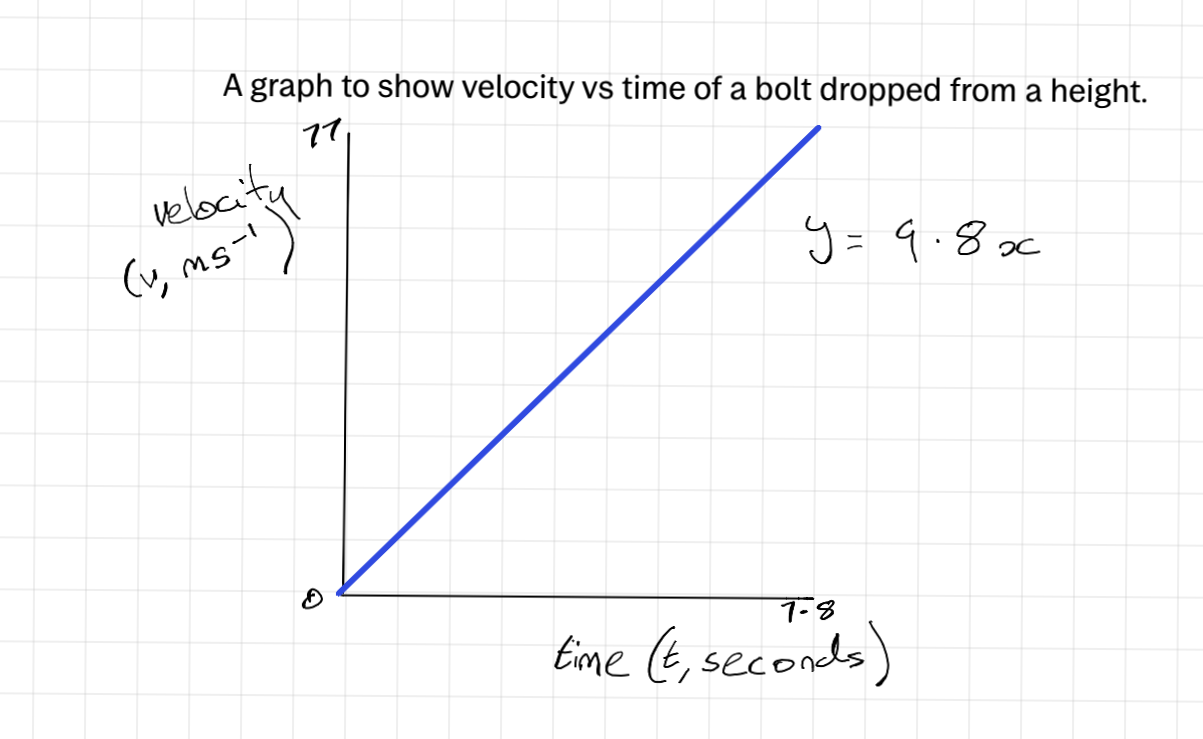
\includegraphics[scale=0.25]{question_5_b.png}

\end{question}

%%%%%%%%%%%Question 6

\begin{question}

\[v_{0}=\SI{0}{meter\per\second}, \quad x_{0}=\SI{0}{\meter}, \quad v_{1}=\SI{9}{\meter\per\second}, \quad x_{1}=\SI{30}{\meter}\]

\qpart

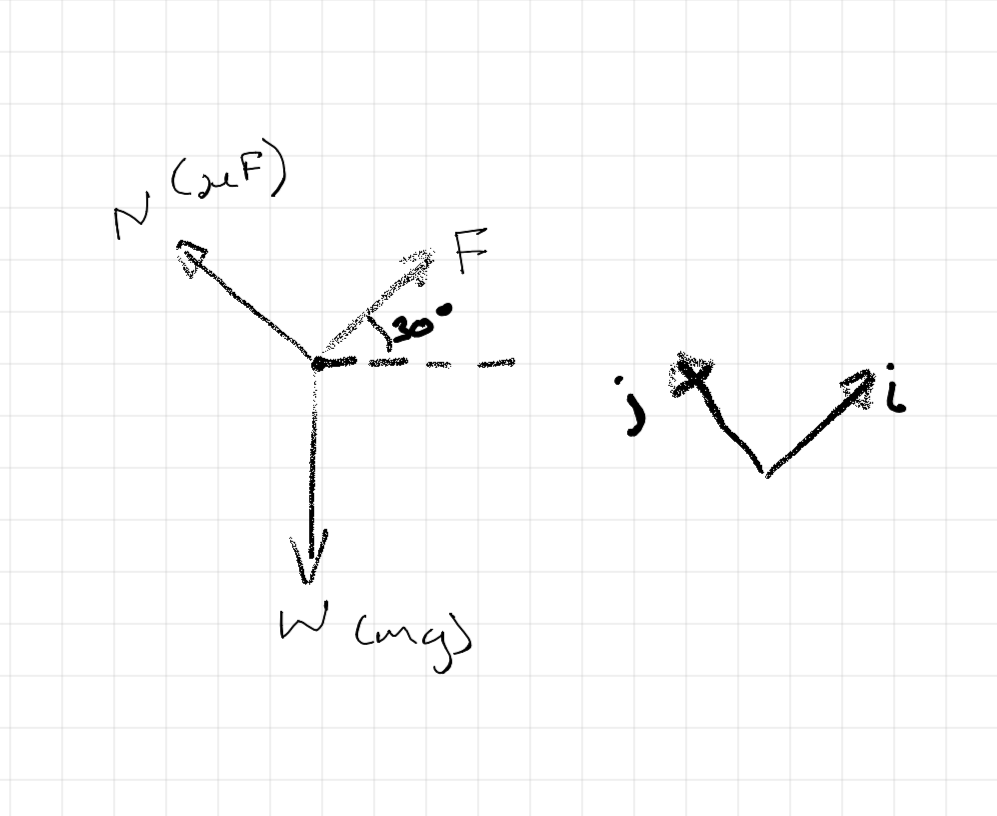
\includegraphics[scale=0.25]{question_6_a.png}

\begin{align*}
\stext{Using}
  v_{1} &= v_{0} + at\\[8pt]
  9 &= at\\[8pt]
\stext{and}
  x_{1} &= v_{0}t + \frac{1}{2}at^{2}\\[8pt]
  30 &= \frac{1}{2}at^{2}\\[8pt]
  60 &= at^{2}\\[8pt]
\stext{Substituting \( at=9 \)}\\[8pt]
  60 &= 9t\\[8pt]
  t &= \frac{60}{9}\\[8pt]
   &= \frac{20}{3}\\[8pt]
   &= \SI{6.67}{\second}
\stext{and}
  a &= \frac{9}{t}\\[8pt]
  a &= \frac{9}{\frac{20}{3}}\\[8pt]
  a &= \frac{27}{20}\\[8pt]
   &= \SI{1.35}{\meter\per\second\squared}
\end{align*}

\vspace{3cm}

\qpart

\begin{align*}
  \mathbf{F} &= \mu|N|\\[8pt]
  \mathbf{N} &= |N|\\[8pt]
  \mathbf{W} &= -\sin(30)mg-\cos(30)mg\\[8pt]
F_{i} &= \sin(30)mg - \mathbf{F}\\[8pt]
&= \sin(30)mg - \mu|N|\\[8pt]
N_{j} &= \cos(30)mg\\[8pt]
\stext{thus}
F &= \sin30mg - \mu\cos(30)mg\\[8pt]
\stext{\text{And using } \(F=ma\)}\\[8pt]
ma &= \sin(30)mg - \mu\cos(30)mg\\[8pt]
\snote{\text{Divinding through by } \(m\)}\\[8pt]
a &= \sin(30)g - \mu\cos(30)g\\[8pt]
1.35 &= \sin(30)g - \mu\cos(30)g\\[8pt]
\snote{Rearranging}\\[8pt]
\mu\cos(30)g &= \sin(30)g - 1.35\\[8pt]
\mu &= \frac{\sin(30)g - 1.35}{\cos(30)g}\\[8pt]
&= \frac{\sin(30)9.8 - 1.35}{\cos(30)9.8}\\[8pt]
&= \frac{4.9 - 1.35}{8.487}\\[8pt]
&= \frac{3.55}{8.487}\\[8pt]
&= 0.418\ldots\\[8pt]
&= 0.42\\[8pt]
\snote{to 2 s.f.}
\end{align*}

\end{question}

%%%%%%%%%%%%Question 7

\begin{question}

\qpart

The vector expression for the acceleration is
\[
\mathbf{a} = -g\mathbf{j}
\]

\vspace{1cm}

\qpart

The initial velocity vector is
\[
\mathbf{v}_0 = 12\cos(50^\circ)\,\mathbf{i} + 12\sin(50^\circ)\,\mathbf{j}
\]

\begin{align*}
\stext{Integrating the acceleration vector to find the velocity vector:} \\[8pt]
\mathbf{v}(t) &= \int \mathbf{a}\,\dd{t }\\
              &= \int -g\mathbf{j}\,\dd{t} \\
              &= -gt\,\mathbf{j} + \mathbf{C}_1
\end{align*}

\begin{align*}
\stext{Using the initial velocity to find the constant of integration:} \\[8pt]
\mathbf{v}(0) &= \mathbf{v}_0 \Rightarrow \mathbf{C}_1 = \mathbf{v}_0 \\[8pt]
\stext{Thus, the velocity vector is:} \\[8pt]
\mathbf{v}(t) &= \mathbf{v}_0 - gt\,\mathbf{j}
\end{align*}

\begin{align*}
\stext{Integrating the velocity vector to find the position vector:} \\[8pt]
\mathbf{r}(t) &= \int \mathbf{v}(t)\,\dd{t} \\
              &= \int \left( \mathbf{v}_0 - gt\,\mathbf{j} \right)\dd{t} \\
              &= \mathbf{v}_0 t - \frac{1}{2}gt^2\,\mathbf{j} + \mathbf{C}_2
\end{align*}

\begin{align*}
\stext{Taking the initial position as the origin:} \\[8pt]
\mathbf{r}(0) &= \mathbf{0} \Rightarrow \mathbf{C}_2 = \mathbf{0} \\
\stext{Therefore}
\mathbf{r}(t) &= \mathbf{v}_0 t - \frac{1}{2}gt^2\,\mathbf{j}
\end{align*}

\begin{align*}
\stext{Substituting the expression for \(\mathbf{v}_0\):} \\[8pt]
\mathbf{r} &= \left(12t \cos(\ang{50})\right) \mathbf{i}
+ \left(12t \sin(\ang{50}) - \frac{1}{2}gt^2\right)\mathbf{j}
\snote{(as required)}
\end{align*}

\vspace{3cm}

\qpart
\qsubpart

Given the position vector \(\mathbf{r}\) is from the orign, we want to find the time \(t\)
for which the \(\mathbf{j}\)-component is \(-1.5\), that is,

\marginnote{The quadratic formula \[x = \frac{-b\pm\sqrt{b^{2-4ac}}}{2a}  \]}

\begin{align*}
12t \sin(\ang{50}) - \frac{1}{2}gt^2 &= -1.5\\[8pt]
\stext{Rewriting}\\[8pt]
-\frac{1}{2}gt^{2} + 12t \sin(\ang{50}) + 1.5 &= 0\\[8pt]
\stext{This is a quadratic equation in \(t\):}\\[8pt]
t &= \frac{-12\sin(50) \pm\sqrt{(12\sin(50)^2-4(-\frac{1}{2}g)(1.5))}}{2(-\frac{1}{2}g)}\\[8pt]
&= \frac{-12\sin(50) \pm \sqrt{(12\sin(50))^2+\frac{147}{5}}}{-g}\\[8pt]
&= -0.151\ldots \text{ and } 2.027\ldots\\[8pt]
\stext{since we can reject the negaive value for time, we have}\\[8pt]
&= 2.027\ldots\\[8pt]
&= \SI{2.0}{\second}\\[8pt]
\snote{to 2 s.f.}
\end{align*}

\vspace{3cm}

\qsubpart

The horizonal distance traveled by the ball is given by the \(\mathbf{i}\)-component of 
the position vector \(\mathbf{r}\) at time \(t\):

\begin{align*}
\mathbf{r}_{\mathbf{i}} &= 12t\cos(50)\mathbf{i}\\[8pt]
\stext{Substituting \(t = 2.027\ldots\)}  \\[8pt]
&= 12(2.027\ldots)\cos(50)\mathbf{i}\\[8pt]
&= 15.635\dots\\[8pt]
&= \SI{16}{\meter}\\[8pt]
\snote{to 2 s.f.}
\end{align*}

\end{question}

%%%%%%%%%%%%Question 8

\begin{question}

\[ \mathbf{A} = \begin{pmatrix}
  5 & 6\\
  18 & 2
\end{pmatrix} \]

\qpart

The determinant of matrix \(\mathbf{A}\) is given by:
\begin{align*}
\det(\mathbf{A}) &= 5 \cdot 2 - 6 \cdot 18\\[8pt]
&= 10 - 108\\[8pt]
&= -98
\end{align*}

The trace of matrix \(\mathbf{A}\) is given by the sum of the diagonal elements:
\begin{align*}
\text{tr}(\mathbf{A}) &= 5 + 2\\[8pt]
&= 7
\end{align*}

\marginnote{The characteristic equation of a \(2 \times 2\) matrix \(\mathbf{A}\) is given by:
\[ \lambda^{2} - (tr \mathbf{A})\lambda + \det\mathbf{A} = 0\]
where \(\lambda\) is the eigenvalue.}

Hence, the characteristic equation of matrix \(\mathbf{A}\) is:
\begin{align*}
\lambda^{2} - 7\lambda - 98 &= 0\\[8pt]
(\lambda-14)(\lambda+7) &= 0\\[8pt]
\stext{Hence the eigenvalues are:}\\[8pt]
\lambda_{1} &= 14\\[8pt]
\stext{and}\\[8pt]
\lambda_{2} &= -7
\end{align*}

\vspace{3cm}

The corresponding eigenvectors can be found by solving the equation:
\[(\mathbf{A} - \lambda \mathbf{I})\mathbf{v} = \mathbf{0}\]

\begin{align*}
\begin{pmatrix}
  5 - \lambda & 6\\
  18 & 2 - \lambda
\end{pmatrix}
\begin{pmatrix}
  x\\
  y
\end{pmatrix}
&= \begin{pmatrix}
  0\\
  0
\end{pmatrix}\\[8pt]
\stext{For } \lambda_{1} = 14:\\
\begin{pmatrix}
  5 - 14 & 6\\
  18 & 2 - 14
\end{pmatrix}
\begin{pmatrix}
  x\\
  y
\end{pmatrix}
&= \begin{pmatrix}
  -9 & 6\\
  18 & -12
\end{pmatrix}
\begin{pmatrix}
  x\\
  y
\end{pmatrix}
= \begin{pmatrix}
  0\\
  0
\end{pmatrix}\\[8pt]
\stext{This gives the system of equations:}\\[8pt]
-9x + 6y &= 0\\[8pt]
18x - 12y &= 0\\[8pt]
\stext{Hence}
-9x +6y &= 18x -12y\\[8pt]
\stext{Rearranging gives}\\[8pt]
-27x + 18y &= 0\\[8pt]
18y &= 27x\\[8pt]
2y &= 3x\\[8pt]
\stext{This gives us the eigenvector:}\\[8pt]
\begin{pmatrix}
  2\\
  3
\end{pmatrix}
\stext{For } \lambda_{2} = -7:\\
\begin{pmatrix}
  5 - (-7) & 6\\
  18 & 2 - (-7)
\end{pmatrix}
\begin{pmatrix}
  x\\
  y
\end{pmatrix}
&= \begin{pmatrix}
  12 & 6\\
  18 & 9
\end{pmatrix}
\begin{pmatrix}
  x\\
  y
\end{pmatrix}
= \begin{pmatrix}
  0\\
  0
\end{pmatrix}\\[8pt]
\stext{This gives the system of equations:}\\[8pt]
12x + 6y &= 0\\[8pt]
18x + 9y &= 0\\[8pt]
\stext{Hence}
12x + 6y &= 18x + 9y\\[8pt]
\stext{Rearranging gives}\\[8pt]
-6x - 3y &= 0\\[8pt]
-3y &= 6x\\[8pt]
-y &= 2x\\[8pt]
\stext{This gives us the eigenvector:}\\[8pt]
\begin{pmatrix}
  -1\\
  2
\end{pmatrix}
\end{align*}

\vspace{3cm}

\qpart

We can express \[ \mathbf{A} = \mathbf{P}\mathbf{D}\mathbf{P}^{-1} \]

Where \( \mathbf{P} \) is \( \begin{pmatrix}
  2 & -1\\
  3 & 2 
\end{pmatrix} \)

and \( \mathbf{D} \) is \( \begin{pmatrix}
  14 & 0\\
  0 & -7
\end{pmatrix} \)

\marginnote{The inverse of a \(2 \times 2\) matrix \(\mathbf{P} = \begin{pmatrix}
  a & b\\
  c & d
\end{pmatrix}\) is given by:
\[ \mathbf{P}^{-1} = \frac{1}{ad - bc}\begin{pmatrix}
  d & -b\\
  -c & a
\end{pmatrix} \]
where \(ad - bc\) is the determinant of \(\mathbf{P}\).}

and \( \mathbf{P}^{-1} \) is the inverse of \( \mathbf{P} \); 
\(\begin{pmatrix}
  \frac{2}{7} & \frac{1}{7}\\
  \frac{-3}{7} & \frac{2}{7}  
\end{pmatrix}\)

Hence, we can write:
\[ \mathbf{A} = \begin{pmatrix}
  2 & -1\\
  3 & 2 
\end{pmatrix}
\begin{pmatrix}
  14 & 0\\
  0 & -7
\end{pmatrix}
\begin{pmatrix}
  \frac{2}{7} & \frac{1}{7}\\
  \frac{-3}{7} & \frac{2}{7}
\end{pmatrix} \]

\vspace{3cm}

\qpart

\[ \mathbf{A}^5 = \mathbf{P}\mathbf{D}^5\mathbf{P}^{-1} \]

\begin{align*}
\mathbf{A}^5 &= \begin{pmatrix}
  2 & -1\\
  3 & 2 
\end{pmatrix}
\begin{pmatrix}
  14^5 & 0\\
  0 & (-7)^5
\end{pmatrix}
\begin{pmatrix}
  \frac{2}{7} & \frac{1}{7}\\
  \frac{-3}{7} & \frac{2}{7}
\end{pmatrix} \\[8pt]
&= \begin{pmatrix}
  2 & -1\\
  3 & 2 
\end{pmatrix}
\begin{pmatrix}
  537824 & 0\\
  0 & -16807
\end{pmatrix}
\begin{pmatrix}
  \frac{2}{7} & \frac{1}{7}\\
  \frac{-3}{7} & \frac{2}{7}
\end{pmatrix} \\[8pt]
&= \begin{pmatrix}
  2 \cdot 537824 + -1 \cdot 0 & 2 \cdot 0 + -1 \cdot -16807\\
  3 \cdot 537824 + 2 \cdot 0 & 3 \cdot 0 + 2 \cdot -16807
\end{pmatrix}
\begin{pmatrix}
  \frac{2}{7} & \frac{1}{7}\\
  \frac{-3}{7} & \frac{2}{7}
\end{pmatrix} \\[8pt]
&= \begin{pmatrix}
  1075648 & 16807\\
  1613472 & -33614
\end{pmatrix}
\begin{pmatrix}
  \frac{2}{7} & \frac{1}{7}\\
  \frac{-3}{7} & \frac{2}{7}
\end{pmatrix} \\[8pt]
&= \begin{pmatrix}
  \frac{1075648 \cdot 2}{7} + \frac{16807 \cdot -3}{7} & \frac{1075648 \cdot 1}{7} + \frac{16807 \cdot 2}{7}\\
  \frac{1613472 \cdot 2}{7} + \frac{-33614 \cdot -3}{7} & \frac{1613472 \cdot 1}{7} + \frac{-33614 \cdot 2}{7}  
\end{pmatrix} \\[8pt]
&= \begin{pmatrix}
  \frac{2151296 - 50421}{7} & \frac{1075648 + 33614}{7}\\
  \frac{3226944 + 100842}{7} & \frac{1613472 - 67228}{7}      
\end{pmatrix} \\[8pt]
&= \begin{pmatrix}
  \frac{2100875}{7} & \frac{1109262}{7}\\
  \frac{3327786}{7} & \frac{1546244}{7}      
\end{pmatrix} \\[8pt]
&= \begin{pmatrix}
  300125 & 158466\\
  475398 & 220892
\end{pmatrix} \\[8pt]      
\end{align*}

\vspace{3cm}

\qpart

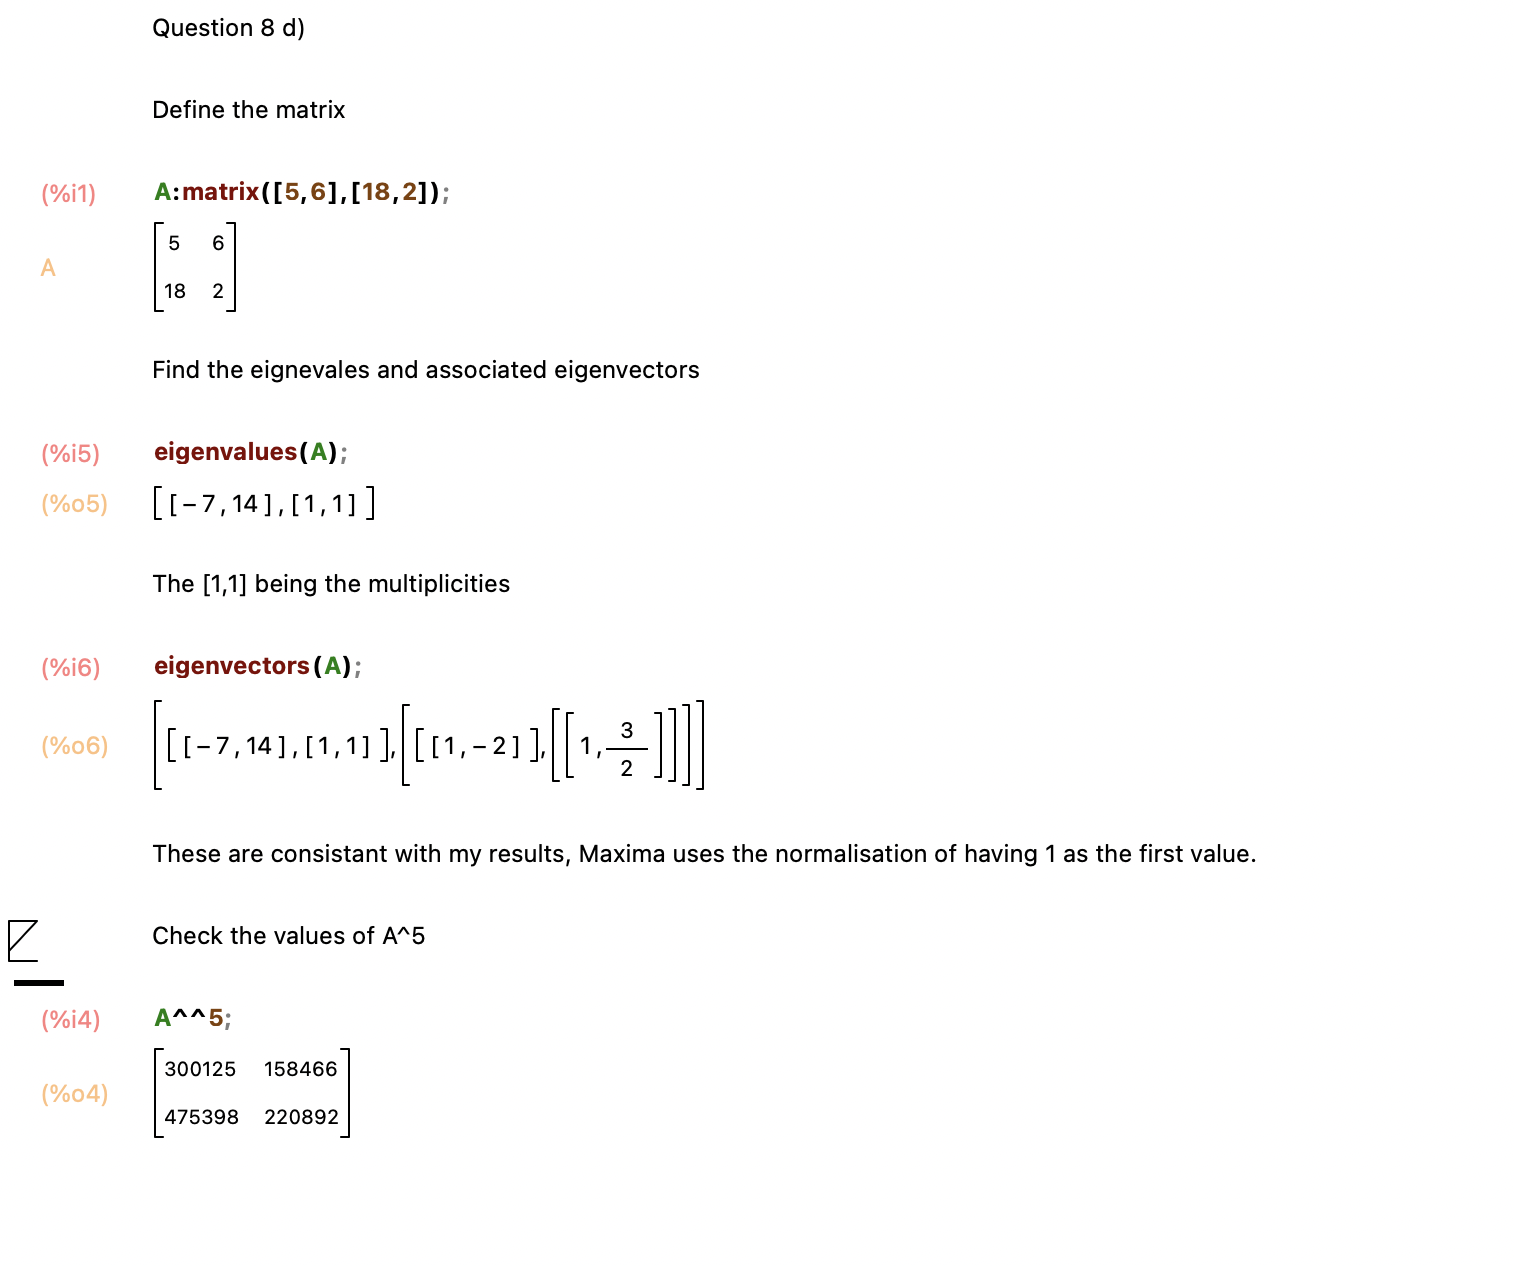
\includegraphics[scale=0.5]{question_8_d.png}

\qpart

\[ \dot{x} = 5x + 6y \]
\[ \dot{y} = 18x + 2y \]

\marginnote{The general solution of a system of linear differential equations is given by:
\[ \mathbf{x} = e^{\lambda_1 t}\mathbf{v}_1 + e^{\lambda_2 t}\mathbf{v}_2 \]
where \(\lambda_1\) and \(\lambda_2\) are the eigenvalues, and \(\mathbf{v}_1\) and \(\mathbf{v}_2\) are the corresponding eigenvectors.}

\begin{align*}
\mathbf{x} &= Ce^{14t}\begin{pmatrix}
  2\\
  3
\end{pmatrix} + De^{-7t}\begin{pmatrix}
  -1\\
  2
\end{pmatrix}\\[8pt]
\stext{hence we can write:}\\[8pt]
x &= 2Ce^{14t} - De^{-7t}\\[8pt]
y &= 3Ce^{14t} + 2De^{-7t}\\[8pt]
\stext{where \(C\) and \(D\) are constants determined by initial conditions.}
\end{align*}

\end{question}

%%%%%%%%%%%%Question 9
\begin{question}

\end{question}

\end{document}